\section{Working with pandas}

\begin{frame}{The idea behind pandas}
  \begin{itemize}
  \item Central concepts: \textcolor{orange}{dataframe} (2D) and \textcolor{orange}{series} (1D)
  \item \emph{Vectorized} operations: apply a function to a whole column or row
  \item Resembles working with R/tidyverse (but: object orientation instead of pipes)
  \end{itemize}
  \pause
Most central ressource: \textcite{McKinney2012}, a book about pandas by the creator of pandas. Updated 3\textsuperscript{rd} edition (2022) freely available online: \url{https://wesmckinney.com/book/}
\end{frame}


\begin{frame}[fragile]{Pandas in the Python ecosystem}
  \begin{itemize}
  \item \emph{The} package that unites everything that fits in a dataframe or in a one-dimensional (time) series
  \item Operates, on the background, with ``basic'' packages such as \texttt{numpy} (stats) or \texttt{matplotlib} (plotting)
  \end{itemize}

\begin{minted}{python}
import pandas as pd
df = pd.DataFrame({"A":[2,3,3,4,3,5], "B":[10,8,9,7,5,5]})
df.corr()
\end{minted}
\vspace{-1cm}
\begin{minted}{python}
import numpy as np
A = [2,3,3,4,3,5]
B = [10,8,9,7,5,5]
np.corrcoef(A,B)
\end{minted}

$\Rightarrow$ The dataframe method \texttt{.corr()} does the same as we could achieve by feeding lists into the numpy function \texttt{corrcoef()}.
\end{frame}




\begin{frame}[fragile]{Pandas in the Python ecosystem}
 Similarily, you can plot directly from pandas\ldots
\begin{minted}{python}
df["A"].hist()
\end{minted}
\ldots or achieve the same by using matplotlib and a list:
\begin{minted}{python}
import matplotlib.pyplot as plt
plt.hist(A)
\end{minted}

\centering

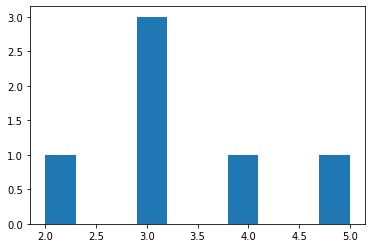
\includegraphics[width=.3\linewidth]{histogram.png}\hfill                           |


\end{frame}


\begin{frame}[standout]
  Pandas simply makes these things easier, and ``to pandas or not to pandas'' is partly a matter of personal preferences. But its really strong point is data wrangling. You really don't want to do \emph{that} without pandas.

\end{frame}




\subsection{Basics of pandas}



\begin{frame}
  \begin{block}{Central concepts}
  \begin{description}[<+>]
  \item[index]\emph{Both} columns and rows have labels -- these are called an index. You can refer to columns and/or rows either by their number or by their label.
  \item[axis] \texttt{axis=0}:  row-wise, \texttt{axis=1}: column-wise
  \item[dtype]columns have a data type (e.g., \texttt{int64}). The generic ``fallback'' option (e.g., mixed types in one column) is simply called \texttt{object}. Not to be confused with\ldots
  \item[object-orientation] Dataframes (and columns) are objects and hence have methods. These methods (typically) return new objects, which have new methods, etc.
  \end{description}
\end{block}
\end{frame}


\begin{frame}[fragile]{Central concepts}
You can use build-in methods\ldots

\begin{minted}{python}
df['radio'].mean()    # returns 3.33
\end{minted}

\ldots or apply a function:

\begin{minted}{python}
import numpy as np

df['age'].apply(np.log)
# if we want to assign the result to a new column, we could do:
df['log(age)'] = df['age'].apply(np.log)
\end{minted}


\end{frame}


\begin{frame}[fragile]{Getting to know your data}
\makebox[\linewidth]{
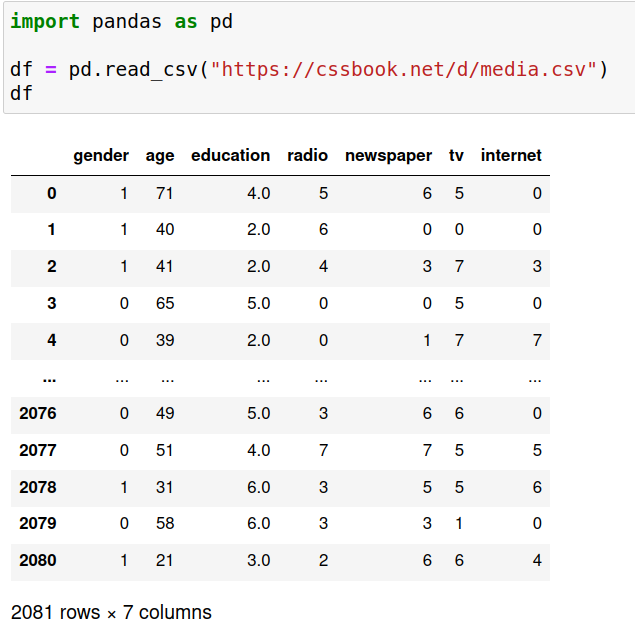
\includegraphics[width=\paperwidth,height=\paperheight,keepaspectratio]{pandas01.png}}
\end{frame}


\begin{frame}[fragile]{Getting to know your data}
\makebox[\linewidth]{
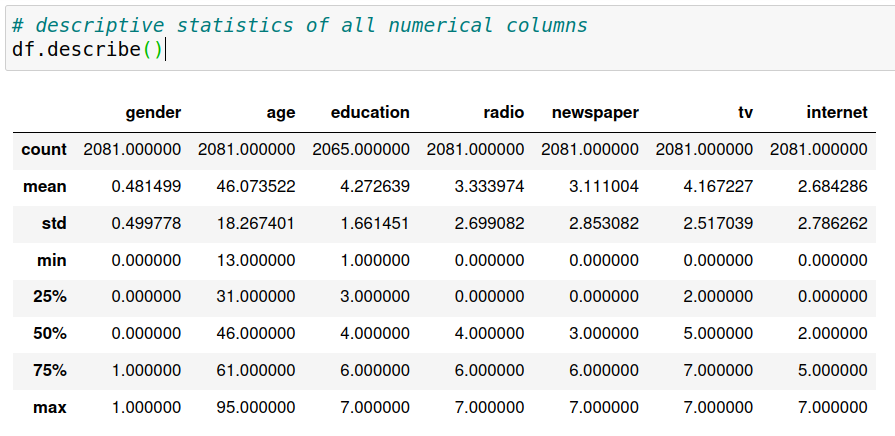
\includegraphics[width=\paperwidth,height=\paperheight,keepaspectratio]{pandas02.png}}
\end{frame}


\begin{frame}[fragile]{Getting to know your data}
\makebox[\linewidth]{
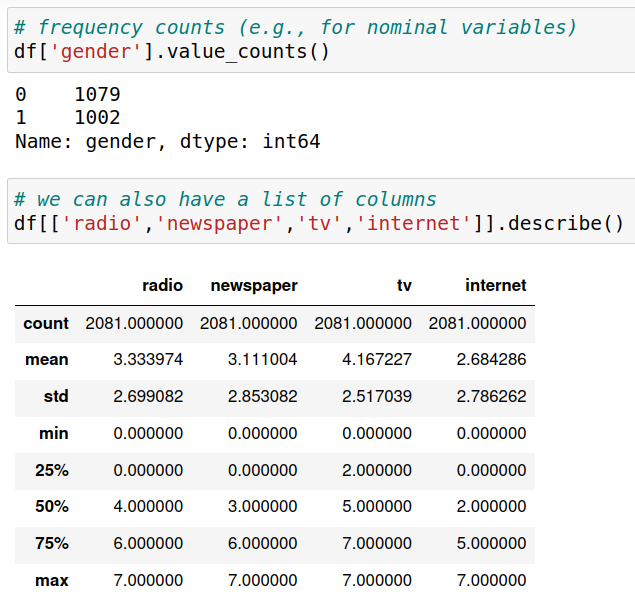
\includegraphics[width=\paperwidth,height=\paperheight,keepaspectratio]{pandas03.png}}
\end{frame}





\question{Any questions so far?}

\begin{frame}[fragile]{Sidenote: standard statistics}
Not the topic of today, but for those interested: Statistical modelling in pandas is a bit ``R-like'' if you use \texttt{statsmodels}:

\begin{minted}{python}
import statsmodels.formula.api as smf

mymodel = smf.ols(formula='internet ~ age + gender +  education', data=df).fit()
mymodel.summary()
\end{minted}    



\end{frame}











%\begin{frame}{}
%More examples here: \url{https://github.com/damian0604/bdaca/blob/master/ipynb/basic_statistics.ipynb}
%\end{frame}



%TODO  WE GAAN HET ZO DOEN


%SLIDES MEER RICHTING BOEK


%WOZ-WAARDE ALS OPDRACHT VOOR LABSESSIE!






\subsection{Data wrangling}




\begin{frame}[fragile]{Recoding values}
There are multiple ways of recoding values: Via the \texttt{.replace()} method or via a function.

\begin{minted}{python}
valuemap = {1:"geen", 7: "WO", 4:"HBO"}
df['education_recoded'] = df['education'].replace(valuemap)  # what's not in the map is kept as-is
\end{minted}


\begin{minted}{python}
def recode_edu(x):
    if x==0:
        return "no"
    elif 1<=x<=4:
        return "low"
    elif x>4:
        return "high"
    
df['education_recoded'] = df['education'].apply(recode_edu)
\end{minted}



\end{frame}





\begin{frame}[fragile]{Subsetting and slicing}
\begin{minted}{python}
df[['gender', 'age']]         # refers to two columns
df.loc[:, ["gender", "age"]]  # the *values* in them
df.iloc[:, [3, 4]]            # use column number instead of label

df.loc[5:10, ["gender", "age"]]  # the values in rows 5--10 in them

df[df.loc[:, 'gender']==0]    # select all rows with females
\end{minted}    
\pause

\emph{\textcolor{orange}{So what's the difference between the approach in line 1 and the \texttt{.loc}/\texttt{.iloc} approach?}}
\end{frame}



\begin{frame}{Subsetting and slicing}
  The difference is between creating a copy and referring to \emph{exactly} the same object itself:
\makebox[\linewidth]{
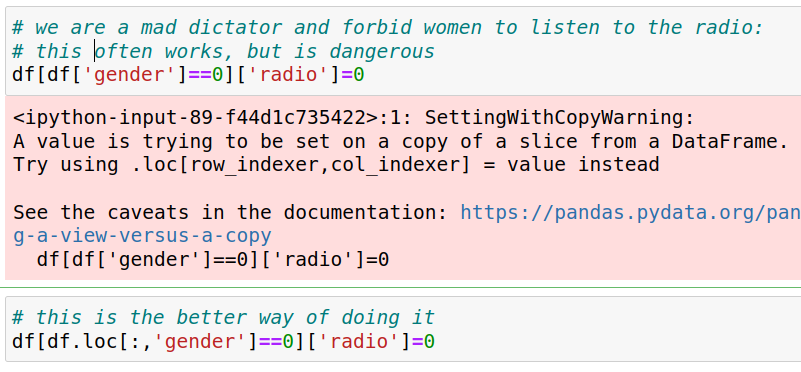
\includegraphics[width=\paperwidth,height=\paperheight,keepaspectratio]{pandas-loc-vs-iloc.png}}
\end{frame}




\question{Do you understand why there is two times \texttt{df} in this expression: \texttt{df[df.loc[:, 'gender']==0]}? Hint: What does the inner part (\texttt{df.loc[:,'gender']==0}) return?  (You may guess!)}




\begin{frame}[fragile]{Subsetting and slicing }
  \begin{block}{A note on hard-coding ``magic numbers}
    \begin{itemize}
    \item Hard-coding ``magic numbers'' like \texttt{687} or \texttt{(0, 5)} should be avoided. Always \emph{calculate} them from your data.
    \item This is a good argument for using \texttt{.loc} over \texttt{.loc}
    \item If you \emph{really} cannot avoid this, define such things a constant at the beginning of your script:)      
    \end{itemize}
  \end{block}

\begin{minted}{python}
INVALID_ROWS = [33, 42, 18]
SPECIAL_ROWS = [120, 111, 230]

# and then, for example, things like:
df.drop(INVALID_ROWS)
newdf = df.iloc[SPECIAL_ROWS, :]
\end{minted}
  
\end{frame}



\subsection{Joining and Merging}

\begin{frame}{Joining and Merging}
\begin{block}{Typical scenario}
	\begin{itemize}
		\item You have two datasets that share one column
		\item For instance, data from \url{www.cbs.nl}: one with economic indicators, one with social indicators
		\item You want to make one dataframe
	\end{itemize}
\end{block}
\end{frame}




{\setbeamercolor{background canvas}{bg=black}
	\begin{frame}[plain]
	\makebox[\linewidth]{
		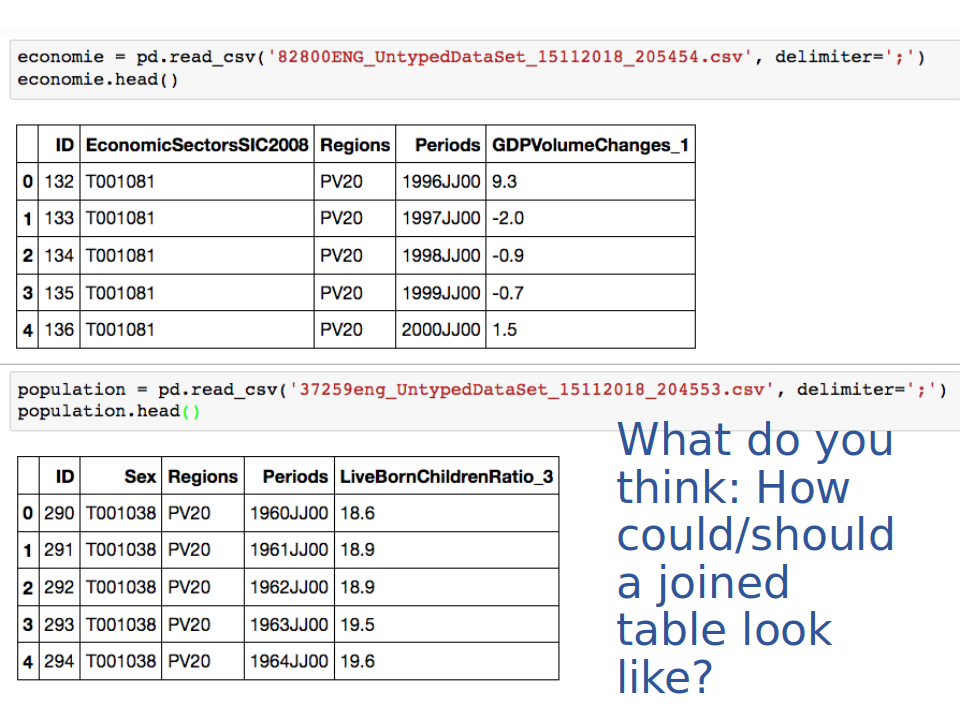
\includegraphics[width=\paperwidth,height=\paperheight,keepaspectratio]{pandas-join1.png}}
\end{frame}
	\begin{frame}[plain]
\makebox[\linewidth]{
	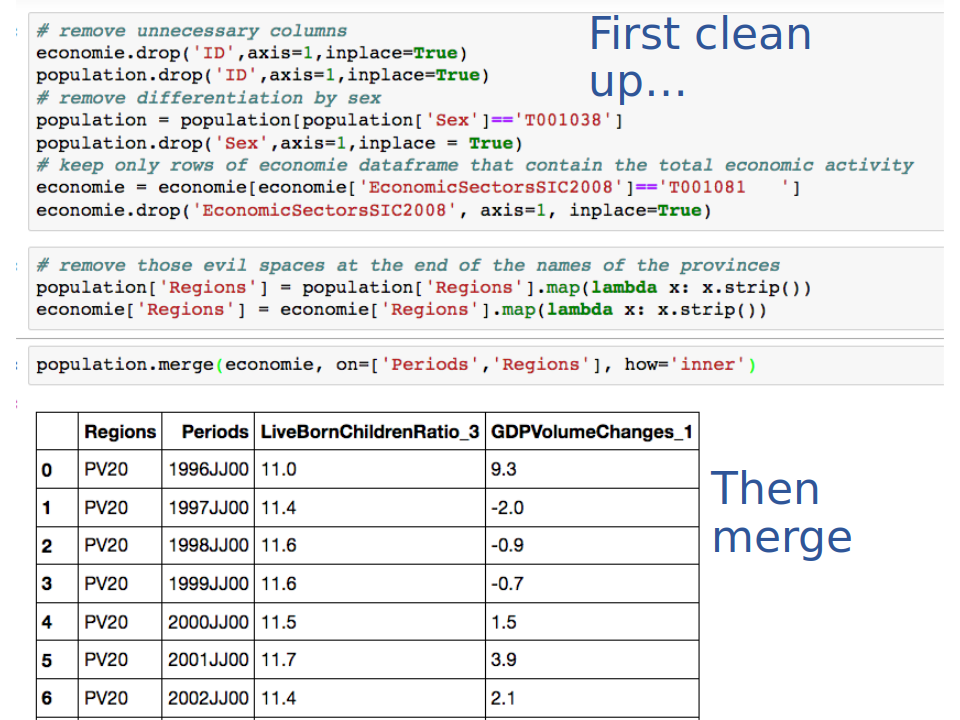
\includegraphics[width=\paperwidth,height=\paperheight,keepaspectratio]{pandas-join2.png}}
\end{frame}
}

\begin{frame}[fragile]{On what do you want to merge/join?}
Standard behavior of.join(): on the row index  (i.e., the row number, unless
you changed it to sth else like a date)
\begin{lstlisting}
df3 = df1.join(df2)
\end{lstlisting}
\pause
But that’s only meaningful if the indices of df1 and df2 mean the same. Therefore you can also join on a column if both dfs have it:
\begin{lstlisting}
df3 = df1.merge(df2, on='Regions')
\end{lstlisting}
\pause
\texttt{.merge()} is the more powerful tool, \texttt{.join()} is a bit easier when joining ion indices.
\end{frame}

\begin{frame}[fragile]{Inner, Outer, Left, and Right}
Main question: What do you want to do with keys that exist only in one of the  dataframes? \\
\pause
\vfill
\texttt{df3 = df1.join(df2, how='xxx')}\\
\vfill

\makebox[\linewidth]{
	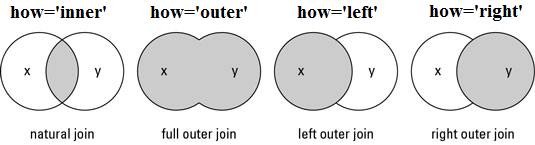
\includegraphics[width=\paperwidth,height=\paperheight,keepaspectratio]{join.png}}
\end{frame}



\begin{frame}[plain]
Aggregation
\end{frame}

\begin{frame}{An example}
\begin{itemize}
	\item Suppose you have two dataframes, both containing information on something  per region per year.
	\item 	You want to merge (join) the two, however, in one of them, the information is also split up by age groups. You don’t want that.
	\item 	How do you bring these rows back to one row? With \texttt{.agg()}!
\end{itemize}

\end{frame}


\begin{frame}{.agg()}
\begin{itemize}[<+->]
	\item Very useful after a \texttt{.groupby()}
	\item Takes a function as argument: \\	\texttt{df2 = df.groupby('region').agg(sum)}
	\item Or multiple functions: \\ \texttt{df2 = df.groupby('region').agg([sum, np.mean])}
	\item $\rightarrow$ yes, you could do \texttt{.describe()}, but \texttt{.agg()} is more flexible	
\end{itemize}
\end{frame}


\begin{frame}[fragile]{An example}
\begin{minted}{python}
import numpy as np

# get all descriptive statistics...
df.groupby("gender")['internet'].describe()

# ... or select specific aggregation functions
df.groupby("gender")['internet'].agg([np.mean, np.std])
\end{minted}


\end{frame}

